% ============================================================
%  Chapter 8 Student Worksheet
%  10 problems per topic · No answer key
%  Compile: pdflatex exfunc_worksheet.tex  (twice)
% ============================================================
\documentclass[12pt, letterpaper]{article}

\usepackage[margin=1in, left=1.2in]{geometry}
\usepackage{amsmath, amssymb, amsthm}
\usepackage{mathtools}
\usepackage{array, booktabs, tabularx}
\usepackage{xcolor}
\usepackage{tcolorbox}
\usepackage{enumitem}
\usepackage{multicol}
\usepackage{tikz}
\usepackage{pgfplots}
\usepackage{fancyhdr}
\usepackage{parskip}
\usepackage[T1]{fontenc}
\usepackage[protrusion=true,expansion=false]{microtype}

\pgfplotsset{compat=1.18}
\tcbuselibrary{skins, breakable}

% ── Colors ──────────────────────────────────────────────────
\definecolor{AccentRed}{RGB}{139,32,32}
\definecolor{Gold}{RGB}{201,150,58}
\definecolor{ExBg}{RGB}{245,240,255}
\definecolor{ExBorder}{RGB}{107,70,193}
\definecolor{LightRule}{RGB}{212,201,176}
\definecolor{PartBg}{RGB}{240,248,255}
\definecolor{PartBorder}{RGB}{30,90,180}

% ── Page style ──────────────────────────────────────────────
\setlength{\headheight}{16pt}
\pagestyle{fancy}
\fancyhf{}
\fancyhead[L]{\small\textbf{Chapter 8} \quad Exponents, Radicals \& Exponential Functions}
\fancyhead[R]{\small\textit{Student Worksheet}}
\fancyfoot[C]{\small$\cdot$\;\thepage\;$\cdot$}
\renewcommand{\headrulewidth}{0.6pt}

% ── tcolorbox: part header ───────────────────────────────────
\tcbset{
  partstyle/.style={
    enhanced, breakable,
    colback=PartBg, colframe=PartBorder,
    leftrule=5pt, toprule=0.8pt, bottomrule=0.8pt, rightrule=0.8pt,
    arc=2pt,
    fonttitle=\large\bfseries\color{PartBorder!80!black},
    attach boxed title to top left={yshift=-2mm, xshift=6mm},
    boxed title style={colback=PartBorder, colframe=PartBorder, arc=2pt},
  }
}
\newtcolorbox{partbox}[1][]{partstyle, title={#1}}

% ── Helpers ──────────────────────────────────────────────────
\newcommand{\nthroot}[2]{\sqrt[\leftroot{-1}\uproot{2}#1]{#2}}
\newcommand{\ws}{\vspace{3.2cm}}          % standard work space
\newcommand{\wss}{\vspace{2.2cm}}         % smaller work space
\newcommand{\ansline}{\underline{\hspace{5cm}}}
\newcommand{\sansline}{\underline{\hspace{3cm}}}

% ── Section rule ────────────────────────────────────────────
\newcommand{\secbar}[2]{%
  \vspace{6pt}
  \noindent\colorbox{AccentRed!10}{%
    \makebox[\dimexpr\linewidth-2\fboxsep\relax][l]{%
      \textbf{\color{AccentRed}#1}\quad{\small\itshape\color{black!70}#2}}}
  \vspace{4pt}
}

% ============================================================
\begin{document}
\hfuzz=1pt  % suppress sub-1pt tcolorbox rounding overflows
% ============================================================

% ── Title block ─────────────────────────────────────────────
\begin{center}
  {\LARGE\bfseries\color{AccentRed} Chapter 8 Practice Worksheet}\\[6pt]
  {\large Exponents, Radicals \& Exponential Functions}\\[10pt]
  \begin{tabular}{@{}lll@{}}
    Name:\;\underline{\hspace{5.5cm}} &
    Date:\;\underline{\hspace{2.8cm}} &
    Period:\;\underline{\hspace{2cm}}
  \end{tabular}\\[6pt]
  \rule{\linewidth}{1.2pt}
\end{center}

\vspace{4pt}

\noindent\fbox{%
  \begin{minipage}{\dimexpr\linewidth-2\fboxsep-2\fboxrule\relax}
  \vspace{2pt}
  \textbf{Key Formulas:}\quad
  $a^m\!\cdot\!a^n=a^{m+n}$\enspace
  $(a^m)^n=a^{mn}$\enspace
  $\dfrac{a^m}{a^n}=a^{m-n}$\enspace
  $a^0=1$\enspace
  $a^{-n}=\dfrac{1}{a^n}$\enspace
  $a^{m/n}=\nthroot{n}{a^m}$
  \vspace{2pt}
  \end{minipage}}

\vspace{10pt}

% ============================================================
%  PART A — Laws of Exponents
% ============================================================
\begin{partbox}[Part A \quad Laws of Exponents \hfill {\normalsize(10 problems)}]
\textit{Simplify each expression completely. Leave all answers with positive exponents.}
\end{partbox}

\vspace{4pt}

\secbar{A1--A5}{Product Rule, Power Rule, Zero \& Negative Exponent}

\begin{enumerate}[label=\textbf{A\arabic*.}, leftmargin=*, itemsep=0pt]

\item $3^2 \cdot 3^5$
\ws

\item $\left(5^2\right)^3$
\ws

\item $7^0$
\wss

\item $4^{-3}$
\ws

\item $\left(2^4\right)^2 \cdot 2^{-3}$
\ws

\end{enumerate}

\secbar{A6--A10}{Quotient Rule, Multi-step Simplification}

\begin{enumerate}[label=\textbf{A\arabic*.}, leftmargin=*, itemsep=0pt, start=6]

\item $\dfrac{x^8}{x^3}$
\ws

\item $\left(3x^2\right)^4$
\ws

\item $\dfrac{a^{-2} \cdot a^5}{a^3}$
\ws

\item $\left(2^3 \cdot 3^2\right)^0$
\wss

\item $\dfrac{\left(2x^3\right)^2}{x^4}$
\ws

\end{enumerate}

\newpage

% ============================================================
%  PART B — Radicals & Rational Exponents
% ============================================================
\begin{partbox}[Part B \quad Radicals \& Rational Exponents \hfill {\normalsize(10 problems)}]
\textit{Convert between radical and rational-exponent form, or evaluate the expression.}
\end{partbox}

\vspace{4pt}

\secbar{B1--B5}{Evaluate using Radicals \& Rational Exponents}

\begin{enumerate}[label=\textbf{B\arabic*.}, leftmargin=*, itemsep=0pt]

\item Evaluate:\quad $\nthroot{10}{1024}$
\ws

\item Write as a radical, then evaluate:\quad $8^{1/3}$
\ws

\item Evaluate:\quad $27^{2/3}$\hfill{\small\itshape Hint: find the cube root first, then square.}
\ws

\item Evaluate:\quad $16^{3/4}$\hfill{\small\itshape Hint: $16=2^4$.}
\ws

\item Evaluate:\quad $\nthroot{5}{32}$
\ws

\end{enumerate}

\secbar{B6--B10}{Convert Between Forms}

\begin{enumerate}[label=\textbf{B\arabic*.}, leftmargin=*, itemsep=0pt, start=6]

\item Write as a rational exponent:\quad $\nthroot{4}{x^3}$
\wss

\item Write in radical notation:\quad $x^{5/6}$
\wss

\item Evaluate:\quad $(-8)^{1/3}$
\ws

\item Simplify:\quad $\dfrac{1}{9^{1/2}}$
\ws

\item Simplify:\quad $(4x^2)^{3/2}$\hfill{\small\itshape Hint: apply the rational exponent to each factor.}
\ws

\end{enumerate}

\newpage

% ============================================================
%  PART C — The Exponential Function y = 2^x
% ============================================================
\begin{partbox}[Part C \quad The Exponential Function $y = 2^x$ \hfill {\normalsize(10 problems)}]
\textit{Answer each question about the exponential function $y = 2^x$.}
\end{partbox}

\vspace{6pt}

\begin{enumerate}[label=\textbf{C\arabic*.}, leftmargin=*, itemsep=0pt]

\item \textbf{Table of values.}\enspace Complete the table for $y=2^x$:

\medskip
\begin{center}
\renewcommand{\arraystretch}{2.0}
\begin{tabular}{|c|c|c|c|c|c|c|c|}
\hline
$x$       & $-3$ & $-2$ & $-1$ & $0$ & $1$ & $2$ & $3$ \\
\hline
$y = 2^x$ & \quad\quad\quad & \quad\quad\quad & \quad\quad\quad & \quad\quad\quad
            & \quad\quad\quad & \quad\quad\quad & \quad\quad\quad \\
\hline
\end{tabular}
\end{center}
\vspace{6pt}

\item \textbf{Sketch the graph.}\enspace Using your table above, graph $y=2^x$ below.
Label at least \textbf{four} points clearly.

\medskip
\begin{center}
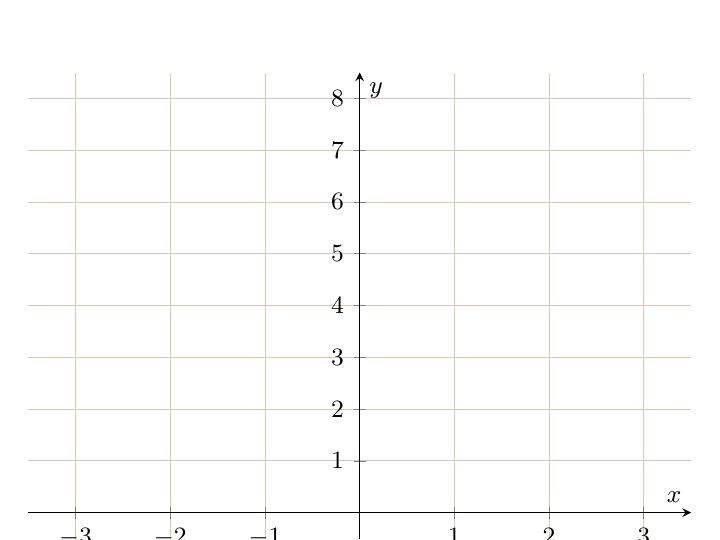
\begin{tikzpicture}
  \begin{axis}[
    width=10cm, height=7.5cm,
    xlabel={$x$}, ylabel={$y$},
    xmin=-3.5, xmax=3.5, ymin=-0.5, ymax=8.5,
    axis lines=center,
    xtick={-3,-2,...,3}, ytick={0,1,...,8},
    grid=both,
    grid style={draw=LightRule, line width=0.3pt},
    tick label style={font=\small},
    label style={font=\small\itshape},
  ]
  \end{axis}
\end{tikzpicture}
\end{center}

\item \textbf{Domain \& Range.}\enspace State the domain and range of $y = 2^x$.

\medskip
\noindent Domain:\;\sansline \qquad Range:\;\sansline
\vspace{0.8cm}

\item \textbf{$y$-intercept.}\enspace What is the $y$-intercept of $y=2^x$? Explain why.

\vspace{2.4cm}

\item \textbf{$x$-intercept.}\enspace Does $y=2^x$ have an $x$-intercept? Explain your answer.

\vspace{2.4cm}

\item \textbf{End behavior.}\enspace Complete the sentences below.

\medskip
\noindent
As $x\to-\infty$,\quad $y\to$ \underline{\hspace{2cm}}\quad because \underline{\hspace{6.5cm}}\\[10pt]
As $x\to+\infty$,\quad $y\to$ \underline{\hspace{2cm}}\quad because \underline{\hspace{6.5cm}}

\vspace{0.6cm}

\item \textbf{Horizontal asymptote.}\enspace True or False: $y=2^x$ has a horizontal asymptote at $y=0$.
Circle one:\quad \textbf{TRUE} \quad / \quad \textbf{FALSE}\\[6pt]
Explain: \underline{\hspace{10cm}}

\vspace{0.6cm}

\item \textbf{Solve for $x$.}\enspace If $2^x = 64$, what is $x$?

\medskip
\textit{Hint: rewrite 64 as a power of 2.}
\ws

\item \textbf{Linear vs.\ Exponential.}\enspace The table below shows values for $y=2x$
(linear) and $y=2^x$ (exponential). Fill in the missing values, then circle which
function grows faster for large $x$.

\medskip
\begin{center}
\renewcommand{\arraystretch}{2.0}
\begin{tabular}{|c|c|c|}
\hline
$x$ & $y = 2x$ & $y = 2^x$ \\
\hline
$1$  & \hspace{2cm} & \hspace{2cm} \\
\hline
$5$  & \hspace{2cm} & \hspace{2cm} \\
\hline
$10$ & \hspace{2cm} & \hspace{2cm} \\
\hline
$20$ & \hspace{2cm} & \hspace{2cm} \\
\hline
\end{tabular}
\end{center}
\medskip
Faster growth for large $x$:\quad $y=2x$ \quad / \quad $y=2^x$ \quad (circle one)

\vspace{0.6cm}

\item \textbf{Connect to Radicals.}\enspace
The point $(10,\,1024)$ lies on $y=2^x$.

\medskip
\noindent
(a)\enspace Express this using \textit{radical notation}:\quad
$\nthroot{\phantom{10}}{\phantom{1024}} = \sansline$

\medskip
\noindent
(b)\enspace Express this using a \textit{rational exponent}:\quad
$(\phantom{1024})^{\phantom{1/10}} = \sansline$

\medskip
\noindent
(c)\enspace Verify your answer to (b) using the Laws of Exponents. Show your work:
\ws

\end{enumerate}


\newpage

% ============================================================
%  ANSWER KEY  (Teacher Copy)
% ============================================================
\begin{center}
  {\LARGE\bfseries\color{AccentRed} Answer Key}\\[4pt]
  {\large Chapter 8 \quad Exponents, Radicals \& Exponential Functions}\\[6pt]
  \rule{\linewidth}{1.2pt}
\end{center}

\vspace{6pt}

% ── Define answer box ──────────────────────────────────────
\tcbset{
  ansstyle/.style={
    enhanced, breakable,
    before upper={\hfuzz=1.5pt},
    colback=green!6, colframe=green!50!black,
    leftrule=4pt, toprule=0.8pt, bottomrule=0.8pt, rightrule=0.8pt,
    arc=2pt,
    fonttitle=\bfseries\color{green!40!black},
    attach boxed title to top left={yshift=-2mm, xshift=6mm},
    boxed title style={colback=green!50!black, colframe=green!50!black, arc=2pt},
  }
}
\newtcolorbox{ansbox}[1][]{ansstyle, title={#1}}

% ── PART A ──────────────────────────────────────────────────
\begin{ansbox}[Part A \quad Laws of Exponents]
\small\setlength{\tabcolsep}{4pt}\renewcommand{\arraystretch}{1.5}
\begin{tabular}{@{} p{22pt} p{0.42\linewidth} p{22pt} p{0.40\linewidth} @{}}
\textbf{A1} & $3^2\cdot3^5 = 3^7 = \mathbf{2187}$
  & \textbf{A2} & $(5^2)^3 = 5^6 = \mathbf{15{,}625}$ \\
\textbf{A3} & $7^0 = \mathbf{1}$
  & \textbf{A4} & $4^{-3} = \dfrac{1}{4^3} = \mathbf{\dfrac{1}{64}}$ \\[6pt]
\textbf{A5} & $(2^4)^2\cdot 2^{-3} = 2^8\cdot 2^{-3} = 2^5 = \mathbf{32}$
  & \textbf{A6} & $\dfrac{x^8}{x^3} = \mathbf{x^5}$ \\[6pt]
\textbf{A7} & $(3x^2)^4 = 3^4\,x^{8} = \mathbf{81x^8}$
  & \textbf{A8} & $\dfrac{a^{-2}\cdot a^5}{a^3}=a^{-2+5-3}=a^{0}=\mathbf{1}$ \\[6pt]
\textbf{A9} & $(2^3\cdot3^2)^0 = \mathbf{1}$\newline
              {\small\itshape Any nonzero base to the 0th power $= 1$.}
  & \textbf{A10} & $\dfrac{(2x^3)^2}{x^4}=\mathbf{4x^2}$ \\[8pt]
\end{tabular}
\end{ansbox}

\vspace{10pt}

% ── PART B ──────────────────────────────────────────────────
\begin{ansbox}[Part B \quad Radicals \& Rational Exponents]
\small\setlength{\tabcolsep}{4pt}\renewcommand{\arraystretch}{1.6}
\begin{tabular}{@{} p{22pt} p{0.42\linewidth} p{22pt} p{0.40\linewidth} @{}}
\textbf{B1} & $\nthroot{10}{1024}=\mathbf{2}$\newline
              {\small\itshape since $2^{10}=1024$}
  & \textbf{B2} & $8^{1/3}=\nthroot{3}{8}=\mathbf{2}$ \\
\textbf{B3} & $27^{2/3}=\!\left(\nthroot{3}{27}\right)^{\!2}\!=3^2=\mathbf{9}$
  & \textbf{B4} & $16^{3/4}=\!\left(\nthroot{4}{16}\right)^{\!3}\!=2^3=\mathbf{8}$ \\
\textbf{B5} & $\nthroot{5}{32}=\mathbf{2}$\newline
              {\small\itshape since $2^5=32$}
  & \textbf{B6} & $\nthroot{4}{x^3}=\mathbf{x^{3/4}}$ \\
\textbf{B7} & $x^{5/6}=\mathbf{\nthroot{6}{x^5}}$
  & \textbf{B8} & $(-8)^{1/3}=\mathbf{-2}$\newline
                  {\small\itshape since $(-2)^3=-8$} \\
\textbf{B9} & $\dfrac{1}{9^{1/2}}=\dfrac{1}{\sqrt{9}}=\mathbf{\dfrac{1}{3}}$
  & \textbf{B10} & $(4x^2)^{3/2}=4^{3/2}\cdot x^3=8x^3\;\Rightarrow\;\mathbf{8x^3}$ \\[6pt]
\end{tabular}
\end{ansbox}

\vspace{10pt}

% ── PART C ──────────────────────────────────────────────────
\begin{ansbox}[Part C \quad The Exponential Function $y=2^x$]

\noindent\textbf{C1.} Table of values:

\smallskip
\begin{center}
\renewcommand{\arraystretch}{1.4}
\begin{tabular}{|c|c|c|c|c|c|c|c|}
\hline
$x$ & $-3$ & $-2$ & $-1$ & $0$ & $1$ & $2$ & $3$ \\
\hline
$y=2^x$ & $\tfrac{1}{8}$ & $\tfrac{1}{4}$ & $\tfrac{1}{2}$ & $1$ & $2$ & $4$ & $8$ \\
\hline
\end{tabular}
\end{center}

\medskip
\noindent\textbf{C2.} Graph should pass through all seven points above, rising steeply to the right and
flattening toward $y=0$ to the left.

\medskip
\noindent\textbf{C3.} Domain: $(-\infty,\,+\infty)$;\quad Range: $(0,\,+\infty)$

\medskip
\noindent\textbf{C4.} $y$-intercept: $(0,1)$, because $2^0=1$.

\medskip
\noindent\textbf{C5.} No $x$-intercept. $2^x>0$ for all real $x$, so the curve never crosses the $x$-axis.

\medskip
\noindent\textbf{C6.} As $x\to-\infty$: $y\to 0$ (approaches asymptote $y=0$).
\quad As $x\to+\infty$: $y\to+\infty$ (exponential growth).

\medskip
\noindent\textbf{C7.} \textbf{TRUE.}\enspace The line $y=0$ (the $x$-axis) is a horizontal asymptote.

\medskip
\noindent\textbf{C8.} $2^x=64=2^6\;\Rightarrow\;x=\mathbf{6}$

\medskip
\noindent\textbf{C9.} Completed table and faster-growth answer:

\smallskip
\begin{center}
\renewcommand{\arraystretch}{1.4}
\begin{tabular}{|c|c|c|}
\hline
$x$ & $y=2x$ & $y=2^x$ \\
\hline
$1$  & $2$  & $2$ \\
$5$  & $10$ & $32$ \\
$10$ & $20$ & $1{,}024$ \\
$20$ & $40$ & $1{,}048{,}576$ \\
\hline
\end{tabular}
\end{center}
\smallskip
Faster growth: $\mathbf{y=2^x}$ (exponential).

\medskip
\noindent\textbf{C10.}
(a)\;$\nthroot{10}{1024}=2$\quad
(b)\;$(1024)^{1/10}=2$\quad
(c)\;$(2^{10})^{1/10}=2^{10\cdot\frac{1}{10}}=2^1=2\;\checkmark$

\end{ansbox}

\end{document}